\chapter{Konzeptualisierung und Refactoring}

\begin{figure}[H]
	\centering
	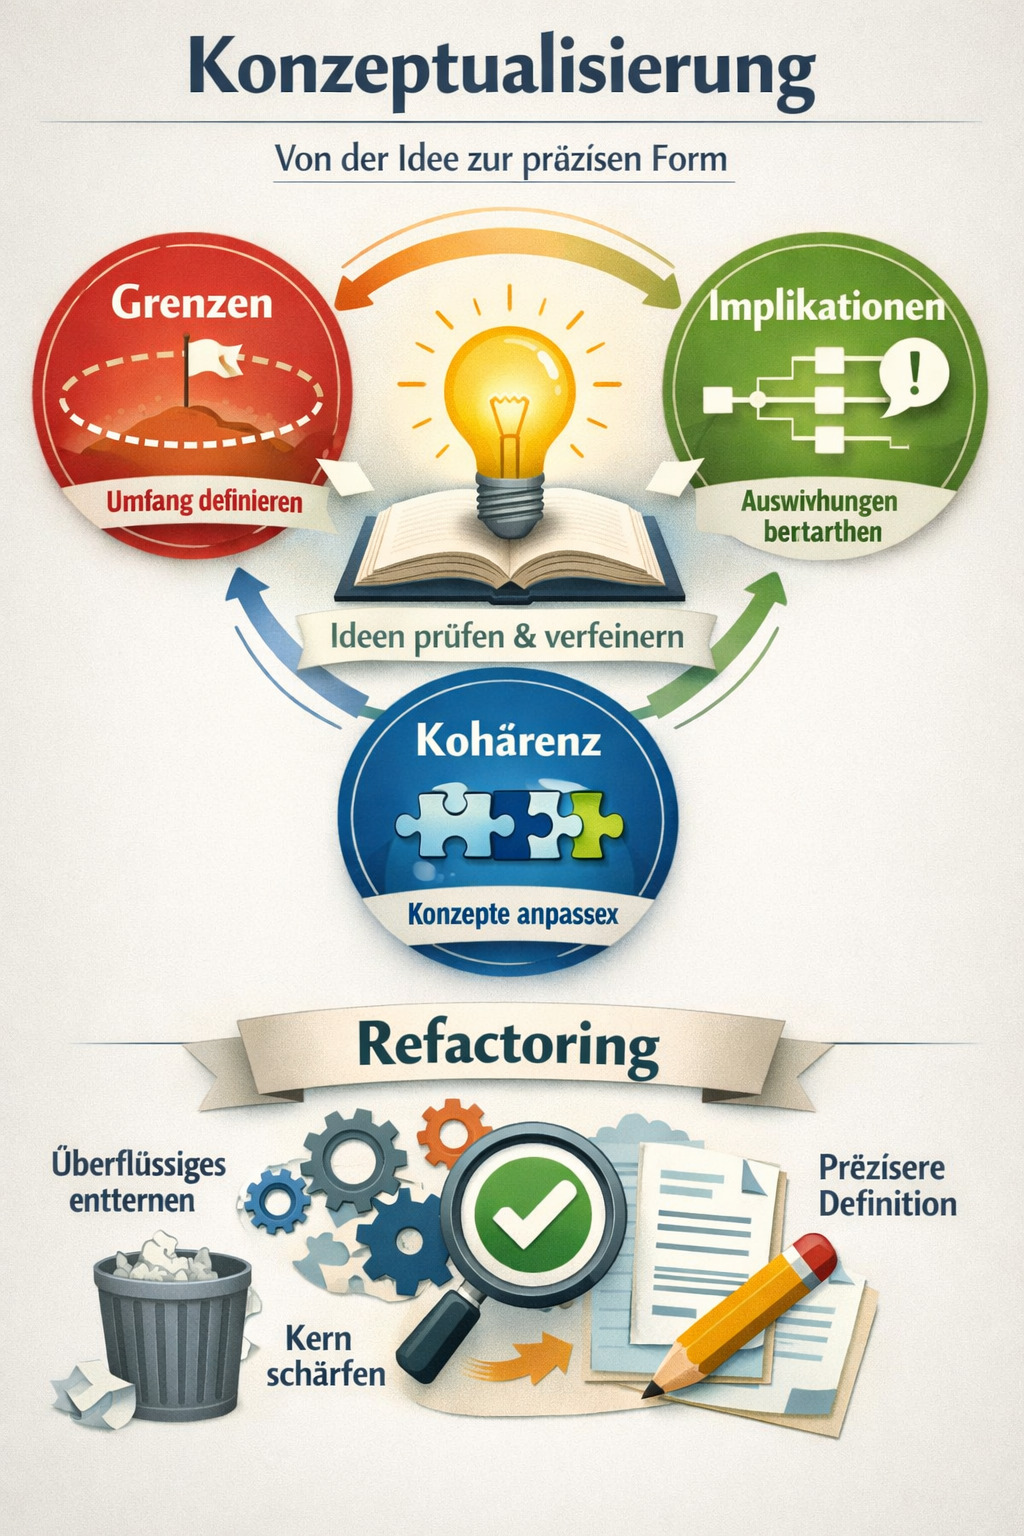
\includegraphics[scale = 0.3]{attachment/chapter_OWN/Scc011.png}
\end{figure} 

\section{Konzeptualisierung}

Der Prozess der Konzeptualisierung – das Verschriftlichen deiner Gedanken – dient dazu, die Grenzen, Implikationen und Kohärenz einer Idee zu erkunden und zu prüfen, um letztlich ihre Tragfähigkeit zu bestimmen.

Obwohl dieser Prozess teilweise zufällig wirken kann, dreht er sich im Kern stets um drei Schlüsselaspekte:
• Grenzen: Sie definieren den Umfang der Idee.
• Implikationen: Sie betrachten die möglichen Ergebnisse und Auswirkungen.
• Kohärenz: Sie bewertet, wie gut sich die Idee in bestehende Konzepte und Rahmenwerke einfügt.

Zusammen sind diese Elemente entscheidend, um ein Konzept zu verfeinern und zu validieren.


\section{Refactoring}

Refactoring bedeutet, ein bereits integriertes und kohärentes Konzept zu verfeinern, um zu seinem Kern vorzudringen. Ziel ist es, Überflüssiges zu entfernen und eine präzisere Beschreibung der Idee zu finden.

Auch in diesem Prozess werden die zentralen Komponenten der Konzeptualisierung – Grenzen, Implikationen und Kohärenz – genutzt, um sicherzustellen, dass das Konzept klar definiert bleibt und die Realität präzise widerspiegelt.
